\section{Uma Linguagem} %------------------------------------------------------
\label{sec:aprendendo} 

\begin{margintable}\vspace{.8in}\footnotesize
  \caption{Sumário da \textsc{Part II}}
  \medskip
  \begin{tabularx}{\marginparwidth}{|X}
    \textbf{\sffamily \textcolor{azulUFRB}{Seção}~\ref{sec:aprendendo}}.    {\sffamily Uma Linguagem} \\
  \end{tabularx}
\end{margintable}

A aquisição de uma linguagem não é algo imediato (para a maioria das pessoas); e,
o \LaTeX{} é uma linguagem, conhecida como \textit{linguagem de marcação}.
Isso implica que há uma \textsf{estrutura} e \textsf{simbologia} características, 
ou seja, é necessário um investimento em tempo e esforço para uma certa fluidez 
na comunicação ou escrita.

Vimos na Subseção~\ref{subsec:latex-word} que o \hologo{LaTeX} é uma linguagem 
que envolve \textit{códigos} e \textit{texto}.
Sua estruturação é diferente de sistemas \textsf{WYSYWYG} (como o Word) e, à
primeira vista, demanda um ``esforço técnico'' maior no início do aprendizado, 
mesmo para documentos simples.
Mas, à medida que a complexidade do documento aumenta, o esforço empregado ao 
usar o \LaTeX{} é menor, quando comparado à sistemas \textsf{WYSYWYG}, para 
produzir o mesmo documento.
A Figura~\ref{fig:latex-vs-word} mostra um vislumbre dessa ideia, embora seja
apenas hipotética.

\begin{figure}[!htbp]
  \centering
  \caption{Complexidade do Documento vs Esforço empregado}
  \label{fig:latex-vs-word}
  \medskip
  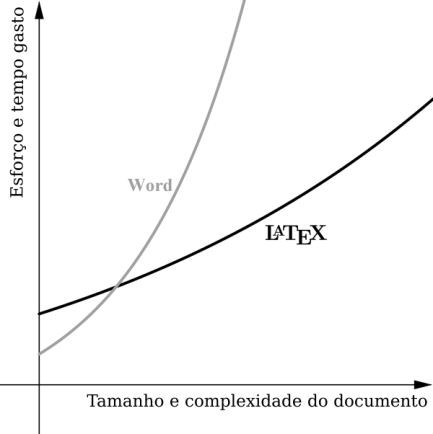
\includegraphics[width = 0.6\linewidth]{figs/latex-vs-word.png}
  
  {\small \textsf{Fonte:} \url{https://latexcfp.wordpress.com/}}
\end{figure}

\begin{marginfigure}
  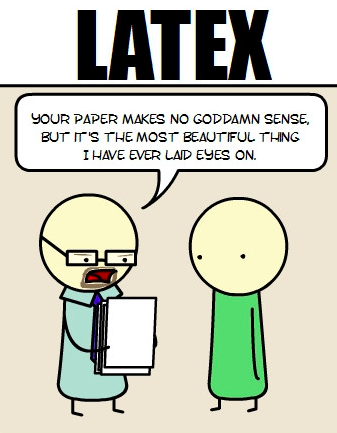
\includegraphics[width = \linewidth]{piada-latex.png}
  
  {
    \sffamily
    \textit{Seu artigo não faz nehum sentido para 
    mim, mas é a coisa mais linda que eu já vi!}
    (Tradução livre e suavizada \emoji{grinning-face-with-sweat})
  }
  
  {\textsf{\textbf{Fonte:}} \hrefB{http://nvisnjic.com/2015/01/13/mathjax-magic.html}{The magic of LaTeX.}}
\end{marginfigure}

Além disso, é notável a beleza da composição tipográfica final, em especial (mas
não necessariamente) quando o documento envolve equações matemáticas.
Como vimos, essa \textsf{beleza} é fruto das mais sofisticadas técnicas empregadas 
nos algorítimos que produzem a saída \textsf{0} ou \textsf{1}, representando, 
respectivamente, ``sem tinta'' ou ``com tinta''.

\subsection{Um pouco sobre a estruturação do LaTeX} %--------------------------

Antes de aprendermos os símbolos pertinentes dessa linguagem, é interessante 
conhecermos um pouco de sua estruturação.
% 
  \subsubsection{Comandos}
% 
Um comando no \LaTeX{} sempre começa com uma barra invertida (``\textbackslash'').
Tal comando pode está inserido em \textsf{modo texto} ou em \textsf{modo matemático}.\mn{
  Existe toda uma sintaxe para o \textsf{modo matemático}, que vamos deixar para
  abordar em outra seção.
}
Por exemplo, quando escrevemos \verb|\LaTeX|, com o ``L'', ``T'' e ``X'' maiúsculos, 
o resultado depois da compilação é: \LaTeX.
Mas, se digitarmos \verb|\Latex|, uma mensagem de erro será mostrada, visto que 
esse comando não vem por padrão definido.

Tal exemplo já nos mostra uma outra característica da estruturação da linguagem 
que estamos conhecendo: ela é \textit{case sensitive}, ou seja, é sensível à
letras maiúsculas e minúsculas.
O comando \verb|\LaTeX| é difernete do comando \verb|\latex|, que é diferente do
comando \verb|\Latex|.
\mn{
  \textsf{\textbackslash LaTeX} $\neq$ \textsf{\textbackslash Latex} $\neq$ \textsf{\textbackslash latex}
}

\begin{atencao}{Atenção!}{\exclamacao}
  Inclusive, essa é uma das grandes fontes de erro de quem está começando no 
  \LaTeX: a digitação de um comando de forma errada é muito comum!
\end{atencao}

Também é importante ressaltar que comandos podem vir acompanhados de 
\textbf{\textsf{argumentos obrigatórios}}, que colocamos entre \textsf{chaves} 
(``\textsf{\{\ldots\}}''); ou de \textbf{\textsf{argumentos opcionais}}, que colacamos 
entre \textsf{colchetes} (``\textsf{[\ldots]}'').

Por exemeplo, o comando \verb|\documentclass| define a \textsf{classe} do 
documento.
O argumento da classe é obrigatório, ou seja, precisamos ``indicar'' ao \LaTeX{}
se estamos usando um \textsf{artigo} (\textit{article}); um \textsf{livro} 
(\textit{book}); um relatório (\textit{report}); uma apresentação (\textit{beamer});
etc.
Além disso, existem vários argumentos opcionais, dentre os quais descato: o 
tamanho da fonte, que por padrão é \textsf{10pt}\mn{ 
  são três opções possíveis nas classes \textit{standard}: \textsf{10pt}, 
  \textsf{11pt} e \textsf{12pt}.
}
; o formato do papel, por exemplo, \textsf{A4}; e a opção de \textit{layout} para
estruturar as margens à impressão em frente e verso: \textsf{twoside}.
Veja como ficaria o comando para a classe \textsf{article}; com tamanho da fonte 
de \textsf{12pt}; definida para um formato de paper \textsf{A4}; e, com a opção 
de imprimir em frente e verso:\mn{
  Note que o comando opcional \textsf{twoside} não ``diz'' para a sua impressora 
  imprimir em ``frente e verso''.
  Apenas configura as margens das páginas para essa opção.
}

\tcboxC{
  \ttfamily \textbackslash documentclass[12pt, a4paper, twoside]\{article\}
}
% 
  \subsubsection{Classe do Documento}
% 
Notem que uma \textsf{classe} possui características instrínsecas: um artigo 
não possui capítulos, mas seções; o que é diferente de um livro, que possui 
essas duas estruturas, por exemplo.
Existem \textsf{classes} que já vem, por padrão, nas distribuições \TeX{} que 
conhecemos e inúmeras outras implementadas pela comunidade de usuários do \LaTeX.

A Tabela~\ref{tab:classes-nativas}, mostra algumas dessas \textsf{classes} 
\textsf{nativas} (também chamadas de \textsf{padrão} ou \textit{standard}).

\begin{margintable}
  \centering
  \caption{Algumas das \textsf{classes} \textit{standard} do \LaTeX}
  \label{tab:classes-nativas}
  \begin{tabular}{lcl}
    \toprule
      \textbs{Classe}  && \textbs{Finalidade} \\
    \midrule
      \textit{article} && artigo     \\
      \textit{book}    && livros     \\
      \textit{report}  && relatórios \\
      \textit{letter}  && carta      \\
    \bottomrule  
  \end{tabular}  
\end{margintable}

\begin{atencao}{Atenção!}{\exclamacao}
  Por conta da limitação de nosso tempo, vamos tangenciar alguns aspectos da 
  linguagem \hologo{LaTeX}, usando apenas a classe \textit{article}.
\end{atencao}

Você já deve ter imaginado que existe uma infinidade de \textsf{classes} para o
\LaTeX, além das nativas.
De fato, há uma comunidade ativa que contribui com seus talentos e disponibilizam,
em sua grande maioria, de forma gratuita muitas funcionalidades/ferramentas que 
facilitam a vida de usuários do \LaTeX.
Dentre essas funcionalidades/ferramentas, estão as \textsf{classes}.
Mas, existem \textbf{pacotes}; aplicativos em java (como o \textsf{arara}); etc.
Geralmente, as \textsf{classes} modificam a estrutura geral de um documento.
Como vimos, um \textsf{artigo} possui uma estrutura diferente de um \textsf{livro},
por exemplo.
O que define essas estruturas são as \textsf{classes}.\en{%
  A extensão do arquivo para uma classe é \textsf{.cls}
}

\begin{atencao}{Atenção!}{\exclamacao}
  Cada classe possui sua sintaxe específica para alguns comandos, porém alguns 
  outros comandos são gerais e servem para a maior parte das classes. 
  Estudaremos apenas esses últimos.
  Caso você queira trabalhar com uma classe diferente da “nativa”, deve 
  verificar o manual para os detalhes.
\end{atencao}

Dentre as classes que não são nativas ao \hologo{LaTeX}, gostaria de destacar:
\nota{
  É bem engraçada, e realista, a descrição do nome abn\TeX:\\ 
  {
    \centering \textit{ABsurd Norms for TeX}.\\
  }
  Por que será, né? \emoji{hand-over-mouth}
}

\begin{description}
  \item[\textas{abn\TeX 2}] Se você pensa em escrever seu Trabalho de Conslusão 
                   de Curso, usandoo \LaTeX, você precisa ler a documentação e 
                   conhecer bem essa classe.
                   Ela, basicamente, fornece um modelo canônico (\textit{template})
                   para várias estruturas de cunho científico, dentro do padrão 
                   da \textsc{abnt} (Associação Brasileira de Normas Técnicas).
                   Você não precisará se preocupar com as configurações de todas
                   aquelas normas em seu texto!
                   Conhecendo os comandos da classe, você só se preocupará com 
                   o \textsf{conteúdo}, não com a \textsf{estrutura}.
                   Inclusive, estou desenvolvendo uma clase para monografia do 
                   curso de Licenciatura em Matemática da UFRB, baseada na classe
                   abn\TeX 2.
                   Ela está disponível lo \textit{link}: 
                   \hrefB{https://github.com/icaro-freire/tccUFRB}{\textsf{tccUFRB.cls}}
  \item[\textas{beamer}] Esta é uma classe para apresentações em \textit{slides} 
                   (chamado também de \textit{frame}, pelos usuários).
                   A qualidade das apresentações é surpreendente. 
                   Principalmente quando a apresentação envolve fórmulas 
                   matemáticas (não distorce como acontece por aí \ldots)!
                   Existem uma infinidade de \textit{templates} (oficiais ou não) 
                   disponíveis que você, certamente, encontrará um que atenda às 
                   suas necessidades.
                   O manual do \textsf{beamer} pode ser visto no \textit{link}:
                   \hrefB
                   {
                     http://tug.ctan.org/macros/latex/contrib/beamer/doc/beameruserguide.pdf
                   }
                   {
                     The \textsc{beamer} \textit{class}
                   }
                   \newline
                   Um \textit{template} de tema claro, extra oficial, que 
                   recomendo para \textsf{beamer} é o 
                   \hrefB{https://github.com/matze/mtheme}{Metropolis};
                   e, um escuro (\textit{dark}): 
                   \hrefB{https://github.com/junwei-wang/beamerthemeNord}{The Nord Beamer Theme.} \\
                   Um pequeno manual, em espanhol, que considero muito prático e 
                   eficiente (principalmente se você não quiser ler as 234~p do 
                   manual oficial) é: 
                   \hrefB{http://metodos.fam.cie.uva.es/~latex/apuntes/apuntes13.pdf}{Presentaciones en \LaTeX\ con Beamer.}
  \item[\textas{exam}] Essa é uma classe para confecção de listas de atividade.
                   Possui um ambiente para soluções; comandos para pontuação nas
                   questões; cria cabeçalhos e rodapés estilizados; etc.
                   Se você é professor e usa fórmulas em suas listas de 
                   atividades, recomendo fortemente ler a documentação dessa 
                   classe \textsf{exam.cls}.
                   Você encontrará o manual nesse \textit{link}:
                   \hrefB{https://ctan.dcc.uchile.cl/macros/latex/contrib/exam/examdoc.pdf}{Using the exam document class}.
                   \newline
                   Baseada nessa classe, desenvolvi (e estou no processo de 
                   atualização) a classe \hrefB{https://github.com/icaro-freire/ativmatUFRB}{ativmatUFRB.cls}.
                   Ela é uma classe não oficial para listas de atividades do 
                   curso de Licenciatura em Matemática, da UFRB.
                   Possui um cabeçalho estilizado com o logo da universidade, bem
                   como comandos e informações que considero úteis num documento
                   desse tipo.
\end{description}

% 
  \subsubsection{Mais sobre Comandos}
% 

Uma pergunta que talvez possa surgir nesse momento: 
\textit{
  se cada comando começa com a ``barra invertida'', qual o comando para 
  representar a própria barra invertida? 
}
  \emoji{thinking}\\
É natural pensarmos em ``\textbackslash\textbackslash'', mas a pergunta surgiria 
novamente: 
\textit{ 
  como representar ``\textbackslash\textbackslash''?
} \emoji{exploding-head}\\
E seguiria uma sequência infinita de pergutas, não?!

Bom, para que essas questões possam ser resolvidas, você deve ter em mente que 
alguns símbolos são \textsf{reservados}, ou seja, há um conjunto de definições 
internas ao próprio \LaTeX. 
Inclusive, símbolos usados em estruturas internas de comandos. 
É o caso de ``\textbackslash'': ele é usado para iniciar qualquer comando no \LaTeX. 
Se você quiser representá-lo textualmente, pode usar \textsf{\textbackslash textbackslash}.
\en{ 
  Veremos que, no modo Matemático, esse mesmo comando pode ser representado 
  simplesmente por \textsf{\textbackslash backslash}.
}

A Tabela~\ref{tab:especial} mostra alguns desses caracteres especiais. 
\begin{table}[!htbp]
  \caption{Caracteres Especiais no \LaTeX}
  \label{tab:especial}
  \centering
  \begin{tabular}{ccl}
    \toprule
      \textbs{Caractere}      && \textbs{Descrição} \\
    \midrule
     \textsf{\textbackslash}  && inicia um comando                                  \\
      \textsf{\%}             && para comentar código                               \\ 
      \textsf{\~{}}           && evita separação de palavras                        \\
      \textsf{\{\;\}}         && delimita códigos                                   \\
      \textsf{\&}             && separa colunas numa tabela                         \\
      \textsf{\#}             && exibe $\textrm{n}^\circ$ de parâmetros num comando \\
      \textsf{\$}             && usado no modo matemático                           \\
      \textsf{\^{}}           && usado para potências                               \\ 
      \textsf{\_{}}           && usado para subíndices                              \\
    \bottomrule
  \end{tabular}
\end{table}

Se você quiser exibir qualquer um deles, (excetuando a \textit{barra invertida},
claro) basta colocar a barra invertida antes dos símbolos!
Por exemplo, se deseja exibir ``10\%'', deve digitar: \textsf{10\textbackslash \%}.

Ainda falando sobre comandos \ldots\ se você for utilizar algum comando interno, 
ou mesmo algum criado por você (sim isso é possível, mas não veremos nesse 
microcurso \emoji{confused-face}), deve ter um cuidado especial com o espaçamento 
de alguma palavra depois do referido comando.
Por exemplo, se formos escrever 
\tcboxC{O \LaTeX\ é sensacional!}
\textbf{não} devemos fazer ``\textsf{O \LaTeX\ é sensacional!}'', visto que a 
saída produzida por esse último comando é:
\tcboxC{O \LaTeX é sensacional!}
Devemos, portanto, colcar ``\textsf{\{\}}'' ou ``\textsf{\textbackslash}'' 
ao final do comando. 
Isso faz com que haja um pequeno espaço entre ele e a próxima palavra. 
Em resumo, você deve fazer alguma das seguintes maneiras:
\begin{enumerate}
  \item[(i)] \textsf{O \textbackslash LaTeX\{\} é sensacional!}
  \item[(ii)] \textsf{O \textbackslash LaTeX\textbackslash\ é sensacional!} 
\end{enumerate}

Gostaria de destacar o uso do comando \textsf{\%} para comentários de código! 
Use-o sempre para lembrar-se de algo ou para organização. 
Ao longo desse texto, esse comando será usado constantemente.

% 
  \subsubsection{Ambientes}
% 

Um agrupamento de comandos peculiar são os \textsf{ambientes} (\textit{environments}). 
Pode ser uma tabela; um ambiente matemático; um ambiente para texto; etc. 
Sempre começará com algum \textsf{\textbackslash begin\{algum-nome\}} e, 
\textbf{obrigatoriamente}, termiar com seu respectivo \textsf{\textbackslash end\{algum-nome\}}. 

\begin{atencao}{Atenção!}{\exclamacao}
  Pode haver a necessidade de ambientes aninhados!
  Por isso, tome cuidado para não esquecer de ``fechar'' um ambiente (com 
  \textsf{\textbackslash end}), inclusive na ordem correta!
  Uma dica é você dar pelo menos dois espaços no início do ambiente interno ao 
  principal.
\end{atencao}

Por exemplo, suponha que você queira escrever o ambiente \textsf{nome-2}, dentro
do ambiente \textsf{nome-1}. 
Então, poderia organizar assim: 

\begin{codigo}{Organizando os ambientes}{\lapis}
\begin{nome-1}
  \begin{nome-2}
    Escreva aqui ...
  \end{nome-2}
\end{nome-1}
\end{codigo}

Um ambiente notável é o \textsf{document}. 
Sem ele não podemos escrever nossos documentos. 
Escrevemos logo depois do comando \Verb|\documentclass|. 
O código abaixo mostra uma estrutura mínima de um texto em \LaTeX. 
Note que usei o comando \textsf{\%} para delimitar partes importantes da 
estrutura no \LaTeX.
Isso é opcional; entretanto, deixa seu código mais arrumado para futuras consultas.
\emoji{wink}

\begin{codigo}{Estrutura mínima para escrever um texto}{\lapis} 
% classe do documento ================================
\documentclass{article}

% início do documento ================================
\begin{document}
% 

Olá! Esse é um pequeno texto em \LaTeX.

% fim do documento ----------------------------------- 
\end{document}
\end{codigo}

%
  \subsubsection{Pacotes}
%
Obviamente, você não precisa ``inventar a roda'' para desenvolver implementações 
no \hologo{LaTeX}.
Muito do que precisamos numa escrita de um artigo que envolva expressões matemáticas, 
já foi pensado e desenvolvido por alguém. 
Essas pessoas, empenharam tempo e dedicação para usar os comandos primitivos do 
\hologo{TeX} ou \hologo{LaTeX} e escreverem seus \textsf{pacotes}.
\nota{
  A sigla \textsf{AmS} vem de \textit{American Mathematical Society}, ou seja, 
  ``Sociedade Americana de Matemética''.
}

Por exemplo, suponha que desejamos escrever expressões matemáticas que envolvam 
\textsf{Matrizes}; \textsf{Integrais}; símbolos da \textsf{Teoria dos Conjuntos};
\textsf{Álgebra}; etc.
Não seria conveniente que a escrita desses comandos seja não conflituosa; 
integrativa e mantenha uma certa harmonia entre eles?
Bom, a \hologo{AmSLaTeX} desenvolveu um conjunto de pacotes essenciais para isso.

\begin{atencao}{Atenção!}{\exclamacao}
  Nessa pseudo-introdução ao \hologo{LaTeX}, os ambientes, fontes e expressões 
  matemáticas serão compostas por meio desses pacotes.
\end{atencao}

Gostaria de destacar, dentre os pacotes da \hologo{AmSLaTeX}, os seguintes:

\begin{description}
  \item[\textsf{amsmath}.] É o principal pacote para expressões e ambientes para 
    escrita matemática.
    Nele podemos enumerar equações; construir matrizes; funções; etc. 
    Realmente é bem vasto e essencial para escrever qualquer texto sério em 
    Matemática.
    Você pode saber mais sobre ele no \text{link}: 
    \hrefB{https://ctan.org/pkg/amsmath}{https://ctan.org/pkg/amsmath}.
  \item[\textsf{amssymb}.] Esse pacote carrega outro muito importante, \textsf{amsfonts}; 
    e, juntos, disponibilizam um conjunto de símbolos e fontes para escrita em 
    Matemática. 
    Dá para escrever $\subset, \varnothing, \triangle, \mathbb{N}, \mathcal{F}$, etc. 
    Você pode saber mais sobre ele no \text{link}: 
    \hrefB{https://ctan.org/pkg/amsfonts}{https://ctan.org/pkg/amsfonts}
  \item[\textsf{amsthm}.] Esse pacote fornece comandos para formatar o estilo, 
    numeração, etc., das Definições, Lemas, Teoremas; Observações, etc.
    Você pode saber mais sobre ele no \text{link}: 
    \hrefB{https://ctan.org/pkg/amsthm}{https://ctan.org/pkg/amsthm}
  \item[\textsf{amscd}.] Pacote com uma linguagem muito simples para escrever 
    \textsf{diagramas comutativos}. \mn{ Um exemplo de diagrama comutativo:\\
      \[
        \begin{CD}
          H   @<f<< H\\
          @V{\psi}VV    @VV{\psi}V\\
          H_1 @<{\psi^\ast (f)}<< H_1
        \end{CD}
      \]
    }
    Você pode saber mais sobre ele no \text{link}: 
    \hrefB{https://ctan.org/pkg/amscd}{https://ctan.org/pkg/amscd}
\end{description}

Falaremos mais sobre esses pacotes de axílio matemático mais à frente; porém, 
é importante destacar que ao longo do tempo, outros pacotes surgiram para complementá-los.
É o caso, por exemplo, do \hrefB{https://ctan.org/pkg/mathtools}{\textsf{mathtool}} 
que, além de carregar o \textsf{amsmath}, ainda disponibiliza correções e novas 
implementações para o mesmo.
Também é notável o pacote \hrefB{https://www.ctan.org/pkg/tikz-cd}{tikz-cd} para 
os diagramas comutativos: simplifica e expande (em muito) o pacote da 
\textsf{amscd}.

Para carregar um pacote ao nosso documento, usamos o comando (Note que alguns 
pacotes podem oferecer opções para configurações.): 

\tcboxC{
  \ttfamily  \textbackslash usepackage[opções]\{nome-do-pacote\}
}

Além disso, também podemos agrupar pacotes. 
Por exemplo, os pacotes citados, da \hologo{AmSLaTeX}, podem ser agrupados assim:

\tcboxC{
  \ttfamily \textbackslash usepackage\{amsmath, amssymb, amsthm\}
}

Você deve imaginar a quantidade exorbitante que exite de pacotes, 
disponíveis para as mais variadas situações no \hologo{LaTeX}: 
desde cifras, tablaturas ou partituras (\hrefB{https://ctan.org/pkg/latex4musicians}{\sffamily \hologo{LaTeX} for Musicians});
songbook (\hrefB{https://ctan.org/pkg/leadsheets}{\sffamily leadsheets}); 
xadrez (\hrefB{https://ctan.org/pkg/texmate}{\sffamily \hologo{TeX}mate}); 
sudoku (\hrefB{https://ctan.org/pkg/sudokubundle}{\sffamily sudokubundle});
labirintos (\hrefB{https://ctan.org/pkg/labyrinth}{labyrinth}); 
etc. (Veja a página sobre  \hrefB{https://ctan.org/topic/games}{\textsf{games}}); até 
construção de gráficos (\hrefB{https://ctan.org/pkg/pgfplots}{\sffamily pgfplots}); 
objetos em 3D (\hrefB{https://texample.net/tikz/examples/tag/3d/}{tikz});
etc. (\hrefB{https://texample.net}{https://texample.net}).

Você pode ver a lista de pocotes disponíveis no \textit{link}:
\nota{
  O \textit{The Comprehensive TeX Archive Network} (CTAN) é um verdadeiro 
  repositório para todo tipo de material em \hologo{TeX}.\\
  Atualmente possui \textsf{6220} pacotes!
}

\tcboxC{
  \hrefB{https://ctan.org/pkg}{https://ctan.org/pkg}
}

Certamente, não precisamos de todos eles num texto!
Tudo dependerá da necessidade e, com o tempo, saberemos selecionar os mais 
adequados aos nossos objetivos.
Todavia, alguns são notáveis, quer por sua simplicidade, quer por suas funcionalidades.
Falaremos sobre eles ao longo desse texto, mas gostaria de descrever parte deles:

\begin{description}
  \item[\hrefB{https://ctan.org/pkg/fontspec}{\sffamily fontspec}] É um pacote 
    essencial para quem usa \hologo{LuaLaTeX} ou \hologo{XeLaTeX}.
    Com ele podemos selecionar as fontes instaladas em nosso sistema operacional, 
    bem como oferece uma codificação adequada à saída das mesmas.\mn{
      Se fôssemos usar o \hologo{pdfLaTeX}, precisaríamos do pacote \textsf{fontenc},
      com codificação \texttt{T1}; além do empacotamento das fontes que desejássemos 
      usar!
    }
  \item[\hrefB{https://ctan.org/pkg/babel}{\sffamily babel}] Ele gerencia as regras 
    tipográficas de mais de 250 idiomas! 
    Quando selecionamos a opção para nosso idioma, esse pacote faz, quando 
    necessário, a hifenação correta das palavras, bem como traduz as estruturas 
    tipográficas características do texto em inglês, na maioria das classes 
    disponíveis.
    Carregamos esse pacote assim:\nota{
      Os caras são realmente criativos! 
      A palavra babel significa ``confundir'' (a tradução vem do hebraico). 
      Há um relato na Bíblia, no Capítulo 11 do livro de Gênesis, sobre a 
      história de uma torre que seria construída pelos seres humanos, quando 
      todos falavam a mesma língua: a chamada \textsf{Torre de Babel}. 
      Se observarmos o contexto do livro, os seres humanos haviam se rebelado 
      contra Deus e, juntos, construiriam essa torre que ``tornaria célebre'' o 
      nome da raça humana corrompida. 
      Deus, então, dispersa esses homens ``confundindo'' (babel) suas linguagens!
      Aí o pessoal do pacote denomina-o por  \textsf{babel}, para retornar à 
      linguagem materna de cada indivíduo. \emoji{upside-down-face}
    }
    \begin{center}
      \Verb|\usepackage[brazil]{babel}|
    \end{center}
  \item[\hrefB{https://ctan.org/pkg/microtype}{\sffamily microtype}] Pacote bem
    sutil que ativa protusão de caracteres e expansão da fonte, além do ajuste 
    entre as palavras, melhorando o espaçamento entre as mesmas.
    Em outras palavras, esse pacote organiza as palavras nos parágrafos de forma 
    harmoniosa, evitanto desalinhamento de texto.
  \item[\hrefB{https://ctan.org/pkg/geometry}{\sffamily geometry}] Fenomenal 
    pacote para ajuste de margens ou papel!
    Apenas como exemplo, para ajustar as margens no padão da ABNT, de um papel 
    A4, podemos fazer:\\
    {\small \Verb|\usepackage[a4paper,top=3cm,left=3cm,bottom=2cm,right=2cm]{geometry}|}
  \item[\hrefB{https://ctan.org/pkg/booktabs}{\sffamily booktabs}] Estilo muito 
   elegante para formatação de tabelas.
  \item[\hrefB{https://ctan.org/pkg/graphicx}{graphicx}] Essencial para inserção
    das figuras no texto.
    Nativamente suporta as extensões \texttt{pdf, png} e \texttt{jpg}.
    Também podemos configurar para que o \LaTeX\ insira apenas as figuras 
    contidas numa pasta, de nome, \texttt{figs}, por exemplo. 
    O carregamento, do pacote é feito como: \Verb|\usepackage{graphicx}|; e a 
    configuração para inserir figuras do diretório \texttt{/figs} como:
    \begin{center}
      \Verb|\graphicspath{{./figs/}}|
    \end{center}
  \item[\hrefB{https://github.com/abntex/biblatex-abnt}{biblatex-abnt}] É um 
    pacote que usa o estilo BibLaTeX (estilo amplo e moderno para compor as 
    bibliografias) para produzir Bibliografia, compatível com as normas da ABNT.
    Usamos o comando \Verb|\usepackage[style=abnt, justify]{biblatex}| para 
    carregarmos o pacote com as normas da ABNT.
    Mas, escrevemos a bibliografia (com comando específicos dessa classe, portanto
    é importantíssimo ler o manual da mesma) num arquivo separado, de extensão 
    \texttt{.bib}, adicionando-o com o comando 
    \Verb|\addbibresource{referencias.bib}| (por nome \textit{referencias}, por 
    exemplo) e exibindo-a com \Verb|\printbibliography| (no arquivo principal).
\end{description}

Agora que comentamos sobre alguns pacotes, vamos organizá-los em nosso arquivo 
\texttt{main.tex}.
Onde colocamos esse comando?

O espaço entre o comando \Verb|\documentclass[]{}| e \Verb|\begin{document}| é 
denominado de \textsf{\textbf{preâmbulo}}.
Nele colocamos as configurações prévias que desejamos fazer em nosso texto (
escolha de fontes; informações sobre título, autor e data; comandos criados por 
você; etc.) e os pacotes que usaremos. \mn{
  Dependendo da distribuição do \TeX\ que você possua em seu computador (caso não 
  use o Overleaf, nem todos os pacotes estão instalados).
  Entretanto, ao carregá-los, geralmente, a instalação é automática.
}

Um arquivo básico seria: 

\begin{codigo}{\texttt{main.tex} (estilizado)}{\lapis}
% classe do documento ================================
\documentclass[12pt]{article}

% preâmbulo ==========================================
% pacotes carregados ---------------------------------
\usepackage{fontspec}
\usepackage[brazil]{babel}

\usepackage[a5paper]{geometry}

\usepackage{mathtools, amsthm, amssymb}
\usepackage{booktabs}

\usepackage{graphicx}
  \graphicspath{{./fig/}}

\usepackage{microtype}

\usepackage[style=abnt, justify]{biblatex}
  \addbibresource{referencias.bib}
% configurações --------------------------------------

% início do documento ================================
\begin{document}
% 

Olá! Esse é um pequeno texto em \LaTeX.

% fim do documento ----------------------------------- 
\end{document}
\end{codigo}

Não coloquei as configurações ainda, pois faremos isso ao longo do texto.
Da mesma forma, ainda não foi colocado o comando para exibir a bibliografia, pois 
falaremos em uma seção específica para ela.
Note, também, que selecionei o tamanho de papel \textsf{A5} para o texto, deixando
as margens no padrão nativo do \LaTeX\ (fica melhor para visualização na tela, 
por estarmos num minicurso online).

\subsection{Arrumando as coisas} %----------------------------------------------

Bom, a proposta é deixar o arquivo principal, \texttt{main.tex}, o mais ``limpo''
possível.

Com efeito, se escrevermos todo o texto, mais as configurações e mais os pacotes;
tudo isso no mesmo arquivo, é possível que haja uma certa desorganização.
Ou, por uma desventura da vida, você apagar de forma descuidada o arquivo, perdendo 
tudo o que escreveu!

Para que situações como a descrita sejam minimizadas, o ideal (no meu entendimento)
é separarmos o conteúdo e incluir essas partes no arquivo principal.
Fazemos essa inclusão por meio do comando:\\

\tcboxC{
  \texttt{\textbackslash input\{nome-do-arquivo.tex\}}
}

Assim, vamos criar, para cada parte de nosso documento, um arquivo de extensão 
\texttt{.tex} e incluí-lo no \texttt{main.tex} por meio do comando \Verb|\input{}|.\mn{
  Futuramente, você pode desenvolver um pacote e salvá-lo numa extensão própria: 
  \texttt{.sty}, que evida possíveis arquivos auxiliares na ``compilação''.
}

Lembrem-se que estamos dentro de um diretório/pasta de nome, por exemplo, 
\texttt{microcurso-EMAT\_LaTeX}.
Então, para orgaizar mais as coisas, vamos criar alguns subdiretórios:
\texttt{figs/}, nele colocaremos \textsc{todas} as \textsf{figuras} utilizadas no 
documento; \texttt{tex/}, nele colocaremos os arquivos \texttt{.tex} que 
incluiremos no arquivo principal.

Inicialmente, vamos criar dois arquivos: \texttt{pacotes.tex} e \texttt{intro.tex}; 
e, à medida que nosso texto for aumentando, criaremos os outros, inclusive o da 
bibliografia (que colocaremos no diretório \texttt{bib/}).

No arquivo \texttt{pacotes.tex}, simplesmente, colocamos os pacotes que desejamos 
carregar (não colocamos \Verb|\documentclass| ou \Verb|\begin{document}|):

\begin{codigo}{\texttt{pacotes.tex}}{\lapis}
\usepackage{fontspec} %-----------> para codificação saída e escolha de fonte
\usepackage[brazil]{babel} %-----------------> suporte para idioma Brasileiro

\usepackage[a5paper]{geometry} %-------------------> configurações de margens
 
\usepackage{mathtools, amsthm, amssymb} %-> para expressões matemáticas e Cia
\usepackage{booktabs} %------------------------> estilo elegante para tabelas
 
\usepackage{graphicx} %---------------------------> para inclusão de gráficos
  \graphicspath{{./fig/}} %-------------------> local onde ficarão as figuras

\usepackage{microtype} %------------------------> para protusão de caracteres

\usepackage[style=abnt, justify]{biblatex} %---> estilo para BibLaTeX para normas ABNT
  \addbibresource{referencias.bib} % adiciona o arquivo .bib
\end{codigo}

Já no arquivo \texttt{intro.tex}, colocaremos nosso texto introdutório:

\begin{codigo}{\texttt{intro.tex}}{\lapis}
Olá! Esse é um pequeno texto em \LaTeX.
\end{codigo}

Agora, no arquivo principal, onde fazemos a composição tipográfica, devemos incluir 
os arquivos que estão em suas respectivas pastas.\mn{
  No \Overleaf{} a compilação no arquivo \texttt{main.tex}, independentemente do 
  arquivo que você estiver editando.
  Basta, apenas, salvar (\texttt{Ctrl + s}).
}
Para carregálos corretamente, usamos os {\textbs{caminhos relativos}}.
Por exemplo, para incluir o arquivo \texttt{pacotes.tex}, que se encontra na pasta 
\texttt{tex/}, devemos usar o comando (note que não precisa escrever a extensão 
do arquivo):\\

\tcboxC{
  \texttt{\textbackslash input\{tex/pacotes\}}
}

Assim, nosso arquivo principal ficaria:\mn{
  Notem que deixei comantado o comando para exibir a bibliografia. 
  Depois de aprendermos a adicionar os comandos no arquivo \texttt{.bib}, 
  desmarcaremos o comentário.
}

\begin{codigo}{\texttt{main.tex}}{\lapis}
% classe do documento ================================
\documentclass[12pt]{article}

% preâmbulo ==========================================
% pacotes carregados ---------------------------------
\input{tex/pacotes}

% configurações --------------------------------------

% início do documento ================================
\begin{document}
% 
  \input{tex/intro} %-------------> texto introdutório
%
%
  %\printbibliography
%
% fim do documento ----------------------------------- 
\end{document}
\end{codigo}

E a organização visua seria algo como a Figura~\ref{fig:diretorios}

\begin{figure}[!htbp]
  \centering
  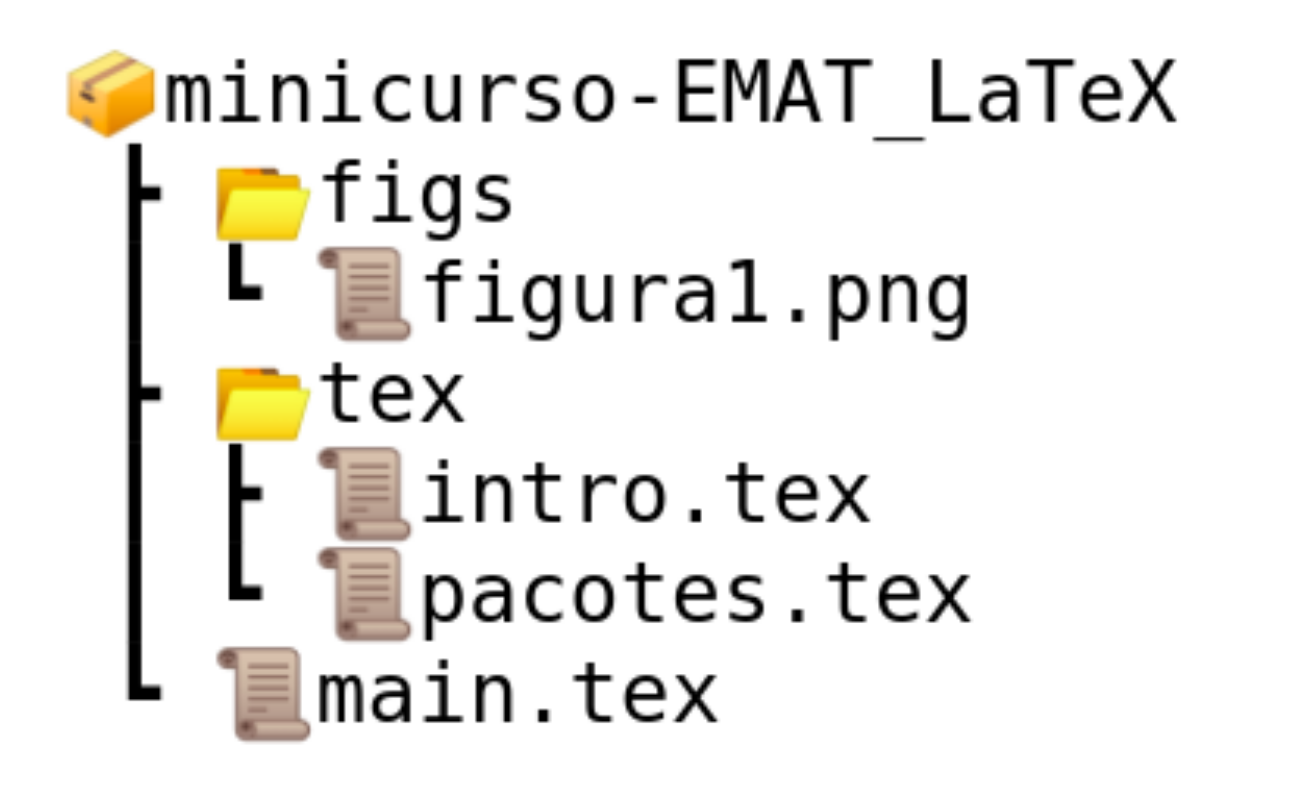
\includegraphics[width=0.45\linewidth]{diretorios}
  \caption{Visualização dos diretórios}
  \label{fig:diretorios}  
\end{figure}

Agora sim, estamos aptos para escrever nosso texto!

%-------------------------------------------------------------------------------
\newpage